\documentclass{article}
\usepackage{enumitem}
\usepackage{graphicx}
\usepackage{float}
\usepackage{array}


\usepackage{geometry}
 \geometry{
 a4paper,
 left=20mm,
 right=20mm
 }


\newlist{legal}{enumerate}{10}
\setlist[legal]{label*=\arabic*.}

\begin{document}
	\begin{figure}
  	
\includegraphics[width=\linewidth]{./images/Logo-PoliMi.jpg}
	\end{figure}
\title{\textbf{RASD}}
\author{Paolo Romeo, Andrea Scotti, Francesco Staccone}
\date{AY 2018-2019}
\maketitle{}
\newpage
\textbf{Table of contents}
	\begin{legal}
 	\item Introduction
  		\begin{legal}
    		\item Purpose
		\item Scope
		\item Definitions, acronyms, abbreviations
		\item Reference documents
		\item Overview	
  		\end{legal}
	\item Overall Description
  		\begin{legal}
    		\item Product perspective
		\item Product functions
		\item User characteristics
		\item Constraints
		\item Assumptions and dependencies
  		\end{legal}
	\item Specific requirements
  		\begin{legal}
    		\item External interface requirements
		\item Functional requirements
		\item Performance requirements
		\item Design constraints
		\item Software system attributes
		\item Other requirements
  		\end{legal}
	\item Formal analysis using Alloy
  	\item Effort spent
	\item References
	\end{legal}
\newpage
	\begin{legal}\bfseries
 	\item Introduction \\
  		\begin{legal}
    		\item Purpose\\
		\\
		{\normalfont The purpose of this document is to fully describe the TrackMe application in terms of goals, functions, requirements and constraints of the system.}
		\\
		\item Scope\\
			\begin{legal}
    			\item Description of the given problem \\
			\item Goals \\
			{\normalfont
				\begin{itemize}
				\item G1) Third parties can monitor the position and the health status of the individuals. \\
				\item G2) Third parties can access the anonymized data of the groups of individuals.\\
				\item G3) The user can accept or refuse the requests concerning the treatment of his/her personal data by the third parties.\\
				\item G4) The third party can subscribe to new data and receive them as soon as they are produced.\\
				\item G5) The user can be recognized by providing a form of identification.\\
				\item G6) The third party can be recognized by providing a form of identification. \\
				\item G7) The user can check the position of the runners at any time during a race.\\
				\item G8) When the health status of the user is in danger, an SOS is launched and an ambulance is sent to the user’s current position.\\
				\item G9) A user can participate to the available races. \\
				\item G10) A third party can organize a race and define the path for the run.\\
				\end{itemize}
				}
			\end{legal}
		\item Definitions, acronyms, abbreviations\\
		\item Reference documents\\
		\item Overview\\
		\end{legal}
	
		
    		
		
	
\newpage
 	\item {Overall description}
  		\begin{legal}
    		\item Product perspective\\
			\begin{figure}[H]
  			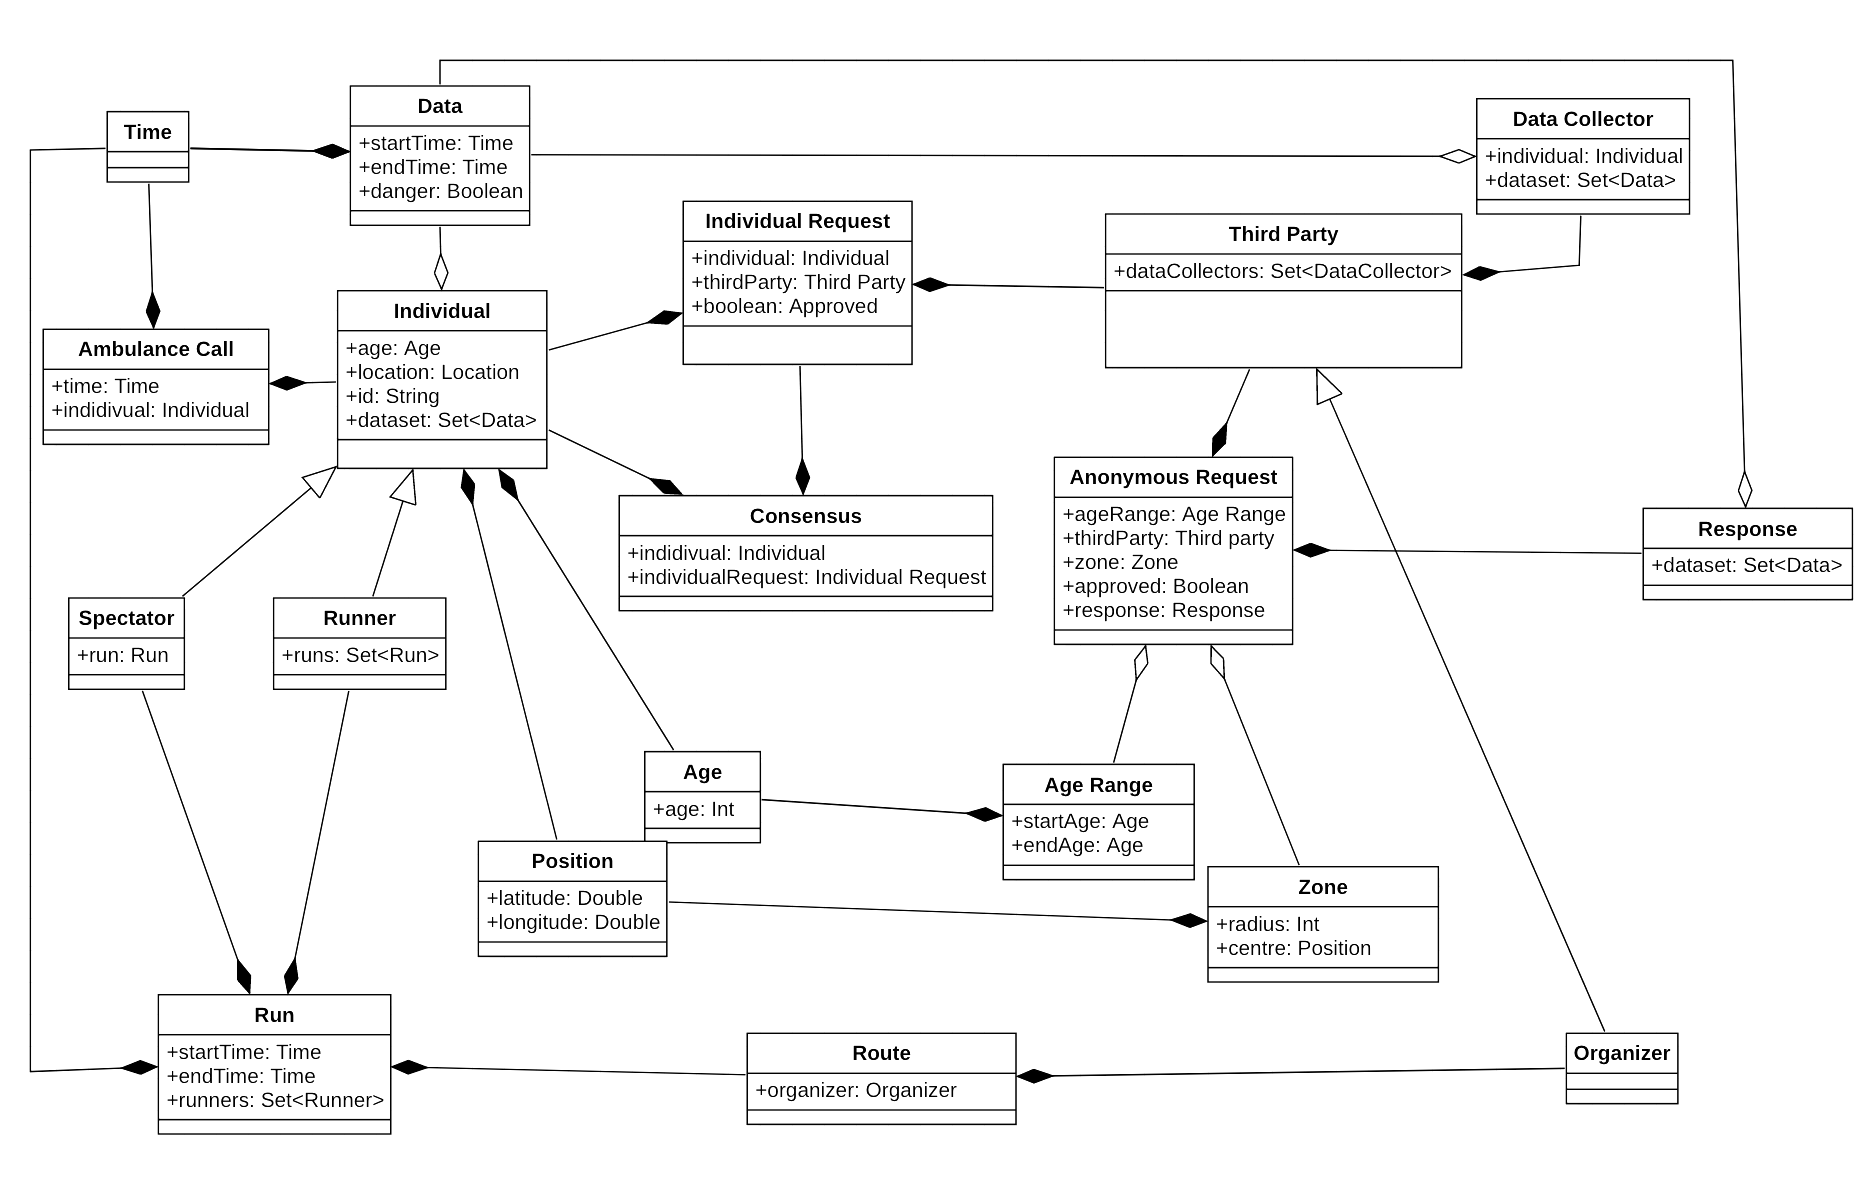
\includegraphics[width=\linewidth]{./images/UML1-0.png}
			\end{figure}
		\item Product functions \\
		\item User characteristics \\
		\item Constraints \\
		\item Assumptions and dependencies \\
			\begin{legal}
    			\item Text assumptions ??? \\
			\item Domain assumptions \\
			{\normalfont
				\begin{itemize}
				\item D1) The measurements of the health status parameters of the individuals are supposed to be reliable.  \\
				\item D2) The position of the individuals is supposed to be reliable.\\
				\item D3) The data acquired from the user’s devices are sent to the mobile application as soon as they are produced.\\
				\item D4) The identification data provided by the users are correct.\\
				\item D5) The identification data provided by the third parties are correct.\\
				\item D6) When an SOS is launched, an ambulance is sent to the position of the user linked to the account that raised the SOS itself. \\
				\item D7) The race takes place in an area with internet coverage and in a compliant track.\\
				\item D8) ?????
				\end{itemize}
			}
			\end{legal}
		\end{legal}
	
\newpage
	\item Specific requirements\\
  		\begin{legal}
		\item External interface requirements\\
			\begin{legal}
    			\item User interfaces \\
				\begin{legal}
    				\item Login or Sign Up 
				\begin{figure}[H]
				\centering
  				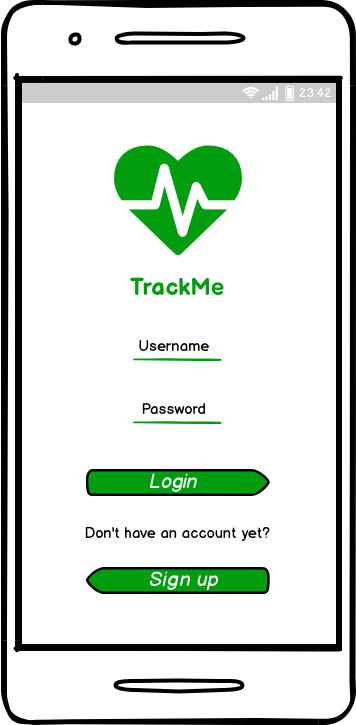
\includegraphics[scale=0.3]{./images/mockups/Login-Sign-up.png}
				\end{figure}
				\item Join a run 
				\begin{figure}[H]
				\centering
  				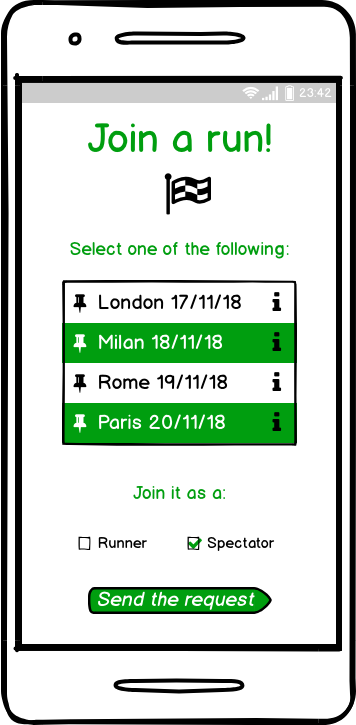
\includegraphics[scale=0.3]{./images/mockups/Join-a-run.png}
				\end{figure}
				\item Define the track of the run 
				\begin{figure}[H]
				\centering
  				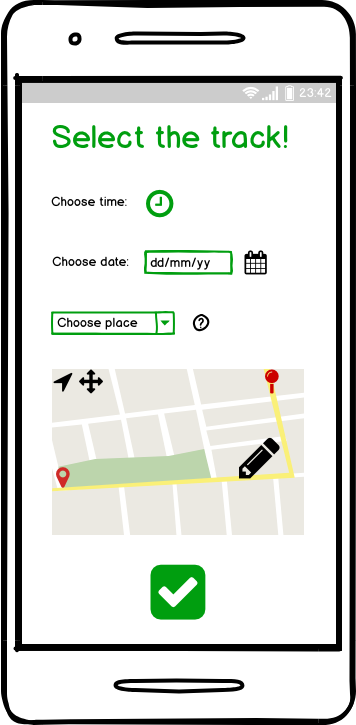
\includegraphics[scale=0.3]{./images/mockups/Path-definition.png}
				\end{figure}
				\item Individual request 
				\begin{figure}[H]
				\centering
  				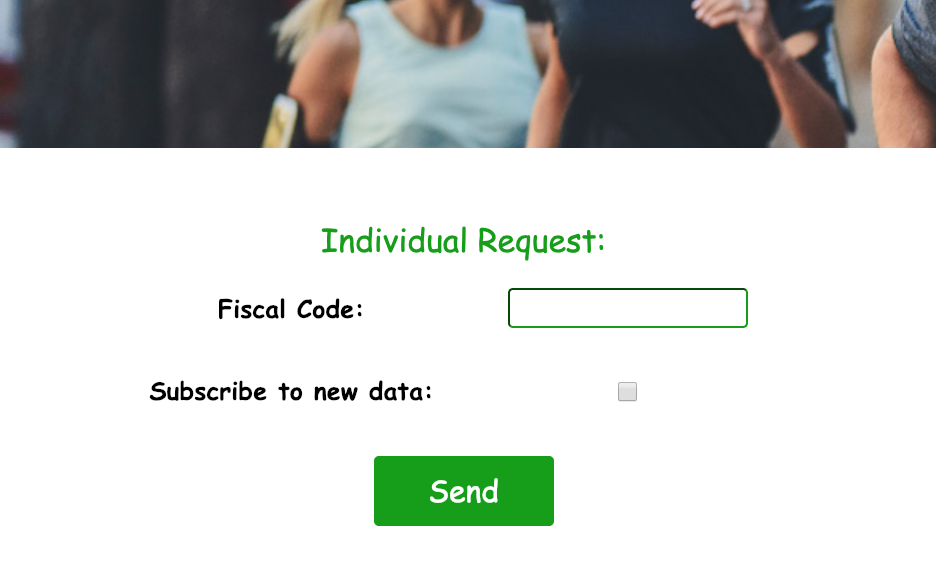
\includegraphics[scale=0.3]{./images/mockups/Individual-request.png}
				\end{figure}
				\item Group request 
				\begin{figure}[H]
				\centering
  				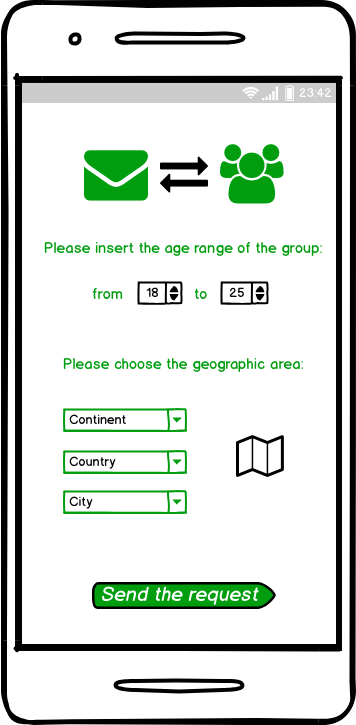
\includegraphics[scale=0.3]{./images/mockups/Group-request.png}
				\end{figure}
				
			\end{legal}
			\end{legal}

    		\item Functional Requirements\\
    		\begin{legal}\bfseries
    			\item Use Case Diagrams
    			\begin{figure}[H]
			  	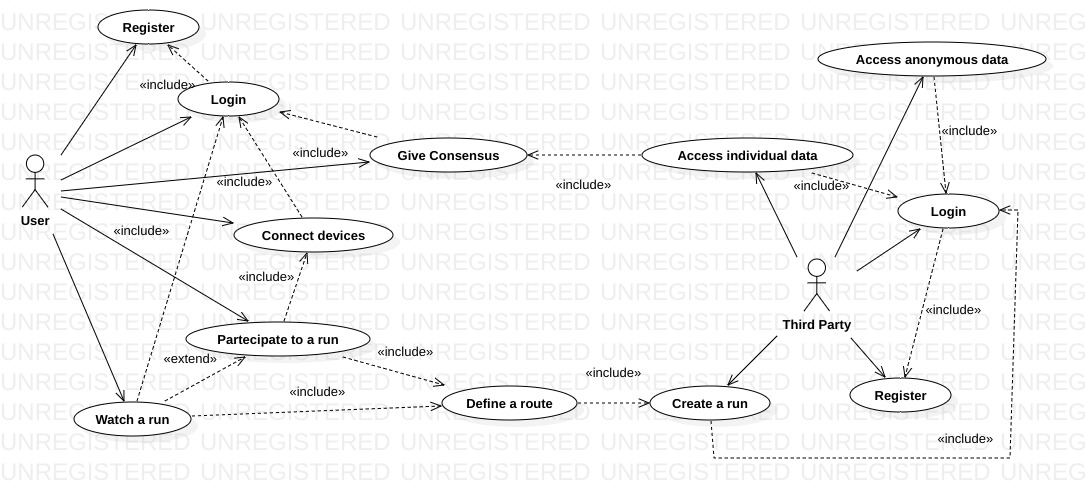
\includegraphics[width=\linewidth]{./images/usecase.jpg}
				\end{figure}
				\begin{tabular}{| m{3.5cm} | m{8cm}| }
				\hline
					Name & Login\\
				\hline
					Actor & Individual\\
				\hline
					Entry Conditions & The user is previously successfully signed up and has the application installed
				on his/her device\\
				\hline
					Event Flows & \begin{enumerate}
									  \item First points
									  \item Second
									  \item Etc.
				\end{enumerate}\\
				\hline
					Exit Conditions & 52\\
				\hline
					Exceptions & 62\\
				\hline
				\end{tabular}
    		\end{legal}
		\end{legal}

	\end{legal}
\end{document}